% ============================================================
%  BISFT — Final IEEE-Style Project Report
%  Business Insights and Sales Forecasting Tool
%  FAST-NUCES Lahore | Spring 2026
% ============================================================
\documentclass[conference]{IEEEtran}
\IEEEoverridecommandlockouts

% ── Packages ─────────────────────────────────────────────────
\usepackage{cite}
\usepackage{amsmath,amssymb,amsfonts}
\usepackage{graphicx}
\usepackage{textcomp}
\usepackage[dvipsnames,svgnames,table]{xcolor}
\usepackage{booktabs}
\usepackage{multirow}
\usepackage{tabularx}
\usepackage{array}
\usepackage{float}
\usepackage{tikz}
\usetikzlibrary{shapes.geometric,arrows.meta,positioning,fit,backgrounds,calc}
\usepackage{pgfplots}
\pgfplotsset{compat=1.18}
\usepackage{listings}
\usepackage[hidelinks,breaklinks]{hyperref}
\usepackage{enumitem}
\usepackage{colortbl}
\usepackage{microtype}

% ── Colour palette ───────────────────────────────────────────
\definecolor{bisftBlue}{RGB}{37,99,235}
\definecolor{bisftGreen}{RGB}{16,185,129}
\definecolor{bisftPurple}{RGB}{124,58,237}
\definecolor{bisftOrange}{RGB}{245,158,11}
\definecolor{bisftRed}{RGB}{239,68,68}
\definecolor{rowgray}{gray}{0.93}
\definecolor{codeBack}{rgb}{0.97,0.97,0.97}

% ── DOI helper ───────────────────────────────────────────────
\newcommand{\doi}[1]{\href{https://doi.org/#1}{doi:#1}}

% ── Code style ───────────────────────────────────────────────
\lstdefinestyle{inline}{
  backgroundcolor=\color{codeBack},
  basicstyle=\ttfamily\scriptsize,
  breaklines=true,
  captionpos=b,
  numbers=left,
  numberstyle=\tiny\color{gray},
  numbersep=4pt,
  showstringspaces=false,
  tabsize=2,
  keywordstyle=\color{bisftBlue}\bfseries,
  commentstyle=\color{OliveGreen},
  stringstyle=\color{BrickRed},
  language=Python,
  frame=single,
  framerule=0.4pt,
  rulecolor=\color{gray!40},
}
\lstset{style=inline}

% ── TikZ reusable styles ─────────────────────────────────────
\tikzset{
  bigbox/.style={
    rectangle, rounded corners=4pt,
    draw=#1!55, fill=#1!12,
    minimum width=7.2cm, minimum height=0.65cm,
    align=center, font=\scriptsize\bfseries,
    text=black
  },
  smallbox/.style={
    rectangle, rounded corners=3pt,
    draw=#1!55, fill=#1!12,
    minimum width=1.45cm, minimum height=0.52cm,
    align=center, font=\tiny\bfseries,
    text=black
  },
  dbbox/.style={
    rectangle, rounded corners=3pt,
    draw=#1!55, fill=#1!12,
    minimum width=2.1cm, minimum height=0.52cm,
    align=center, font=\tiny\bfseries,
    text=black
  },
  astate/.style={
    ellipse,
    draw=bisftBlue!65, fill=bisftBlue!10,
    minimum width=1.6cm, minimum height=0.52cm,
    align=center, font=\tiny\bfseries
  },
  adecision/.style={
    diamond, aspect=2.1,
    draw=bisftOrange!80, fill=bisftOrange!12,
    inner sep=1.5pt,
    align=center, font=\tiny\bfseries
  },
  aaction/.style={
    rectangle, rounded corners=3pt,
    draw=bisftGreen!65, fill=bisftGreen!10,
    minimum width=1.55cm, minimum height=0.5cm,
    align=center, font=\tiny
  },
  myarr/.style={-{Stealth[length=3.5pt,width=2.8pt]}, thick, #1},
}

% ─────────────────────────────────────────────────────────────
\begin{document}

% ══════════════════════════════════════════════════════════════
%  CUSTOM TITLE PAGE  (single column)
% ══════════════════════════════════════════════════════════════
\onecolumn
\thispagestyle{empty}
\begin{center}

{\large\bfseries FAST National University of Computer and Emerging Sciences}\\[3pt]
{\normalsize Department of Computer Science\ \textbullet\ Lahore Campus}

\vspace{0.9cm}
{\color{bisftBlue}\rule{\textwidth}{1.8pt}}\\[5pt]

{\LARGE\bfseries Business Insights and Sales Forecasting Tool}\\[6pt]
{\large\itshape BISFT~v2.0 — An AI-Driven Decision Intelligence Platform}\\[5pt]

{\color{bisftBlue}\rule{\textwidth}{1.8pt}}\\[0.7cm]

{\large\bfseries Final Project Report}\\[3pt]
{\normalsize AI Capstone\ /\ Senior Design Project \textbullet\ Spring 2026}

\vspace{1.4cm}

\begin{tabular}{r@{\ \ }l}
  \textbf{Authors}          & Abdullah Arshad\quad\textbf{(23L-2531)}          \\[3pt]
                            & Sohaib Haider\quad\;\textbf{(23L-2519)}           \\[9pt]
  \textbf{Supervisor}       & [Supervisor Name], FAST-NUCES Lahore              \\[9pt]
  \textbf{Submission Date}  & May 2026                                          \\[9pt]
  \textbf{Web Application}  & \href{http://localhost:5173}{\texttt{http://localhost:5173}}       \\[2pt]
  \textbf{REST API}         & \href{http://localhost:8000}{\texttt{http://localhost:8000}}       \\[2pt]
  \textbf{API Docs (Swagger)} & \href{http://localhost:8000/docs}{\texttt{http://localhost:8000/docs}} \\[2pt]
  \textbf{Source Repository}& \href{https://github.com/abdullaharshaddd/business-insights-and-sales-forecasting-tool}%
                              {\texttt{github.com/abdullaharshaddd/bisft}}       \\
\end{tabular}

\vspace{1.8cm}
{\color{bisftBlue}\rule{0.55\textwidth}{0.5pt}}
\vspace{0.6cm}

\begin{minipage}{0.82\textwidth}
\begin{center}{\large\bfseries Abstract}\end{center}
\small
This report presents the design, implementation, and evaluation of the Business Insights and Sales
Forecasting Tool (BISFT), a production-ready, full-stack AI decision-intelligence platform.
The system integrates a \textbf{Random Forest} sales forecasting engine, a deep neural network (DNN)
churn prediction model, an eleven-function deterministic analytics layer, and a LangGraph-powered
multi-agent conversational AI consultant.  The backend is built on \textbf{FastAPI} with
\textbf{PostgreSQL} as the primary relational store and \textbf{ChromaDB} for semantic knowledge
retrieval. A React~18 frontend delivers an interactive business dashboard, a combined sales and
inventory management module, and an AI chat interface.  Evaluated on the Brazilian E-Commerce
(Olist) and UK Online Retail datasets, the Random Forest forecasting model achieves a test
RMSE of 11{,}243 (MAPE~22.4\%, $R^{2}\!=\!0.87$), while the churn DNN yields an AUC-ROC
of~0.82 overall.  The platform provides actionable intelligence across revenue analytics,
customer lifetime value, delivery performance, and geographic market segmentation.
\end{minipage}

\end{center}
\clearpage

% ══════════════════════════════════════════════════════════════
%  IEEE TWO-COLUMN PAPER BODY
% ══════════════════════════════════════════════════════════════
\twocolumn

\title{%
  Business Insights and Sales Forecasting Tool:\\
  An AI-Driven Decision Intelligence Platform%
}

\author{%
  \IEEEauthorblockN{Abdullah Arshad\textsuperscript{\dag}\quad Sohaib Haider\textsuperscript{\dag}}
  \IEEEauthorblockA{%
    \textsuperscript{\dag}Department of Computer Science, FAST-NUCES, Lahore, Pakistan\\
    \texttt{\{23l-2531, 23l-2519\}@lhr.nu.edu.pk}%
  }%
}

\maketitle

\begin{abstract}
This paper presents the BISFT platform, an AI-driven business intelligence system that
unifies a Random Forest revenue forecasting pipeline, a DNN churn predictor, eleven
deterministic analytical tools, and a LangGraph multi-agent AI consultant within a single
full-stack web application.  The system ingests two heterogeneous e-commerce datasets through
a bespoke PostgreSQL ETL pipeline, exposes 15+ REST endpoints via FastAPI, and renders results
through a React~18 dashboard.  The Random Forest model achieves MAPE~22.4\% and
$R^{2}\!=\!0.87$ on the held-out test set; the DNN churn model achieves AUC-ROC~0.82.
The Agentic RAG consultant successfully handles multi-step analytical queries through
coordinated tool use, semantic retrieval, and Llama~3.3~70B synthesis.
\end{abstract}

\begin{IEEEkeywords}
Business Intelligence, Sales Forecasting, Random Forest, Churn Prediction,
Agentic RAG, LangGraph, FastAPI, PostgreSQL, E-Commerce Analytics
\end{IEEEkeywords}

% ─────────────────────────────────────────────────────────────
\section{Introduction}

Data-driven decision-making has become essential for modern e-commerce enterprises.
Organisations accumulate vast transaction histories, customer behaviour records, and logistical
data, yet frequently lack integrated tooling to extract actionable intelligence in real time.
Business analysts navigate fragmented dashboards, manually trigger model retraining, and consult
siloed reports — creating latency between data generation and strategic response.

BISFT addresses this gap through a unified, AI-augmented analytics platform that combines a
deterministic KPI engine, a supervised ML pipeline, and a conversational multi-agent system.
The platform is trained on two publicly available datasets: the Olist Brazilian E-Commerce
dataset~\cite{olist2018} (99{,}441 orders, 2016–2018) and the UCI Online Retail
dataset~\cite{online_retail2015} (541{,}909 transactions, 2010–2011).

The primary contributions of this work are:
\begin{itemize}[leftmargin=*,noitemsep,topsep=2pt]
  \item A production-ready \textbf{Random Forest} forecasting pipeline with 15 engineered
        lag and rolling-window features achieving MAPE~22.4\%, $R^{2}\!=\!0.87$.
  \item A \textbf{DNN churn model} (128-64-32) with RFM feature engineering achieving
        AUC-ROC~0.82.
  \item An \textbf{Agentic RAG} architecture implementing a five-node LangGraph state
        machine orchestrating nine specialised tools and a ChromaDB knowledge base.
  \item A \textbf{thirteen-table PostgreSQL schema} with a complete Python ETL pipeline
        from raw CSV sources.
  \item A \textbf{full-stack web application} covering inventory management, sales analytics,
        real-time KPI dashboards, and a natural-language business consultant.
\end{itemize}

% ─────────────────────────────────────────────────────────────
\section{Problem Statement}

E-commerce businesses generate multi-dimensional transactional data across orders,
customers, sellers, logistics, and payments. Four core challenges motivate BISFT:

\textbf{(P1) Reactive analytics.}
Revenue forecasting is performed ad-hoc, depriving planners of forward visibility for
inventory procurement and campaign scheduling.

\textbf{(P2) Undifferentiated churn management.}
Without automated RFM segmentation and churn scoring, retention initiatives are applied
uniformly rather than targeted at at-risk customer cohorts.

\textbf{(P3) Fragmented tooling.}
Analysts switch between SQL editors, standalone BI tools, Jupyter notebooks, and
spreadsheets for routine business questions, increasing cognitive load and error risk.

\textbf{(P4) Knowledge retrieval latency.}
Institutional knowledge about KPI definitions, historical trends, and recommended
interventions is scattered across documents requiring manual synthesis.

% ─────────────────────────────────────────────────────────────
\section{Objectives}
\begin{enumerate}[leftmargin=*,noitemsep,topsep=2pt]
  \item Design a 13-table relational PostgreSQL schema from two heterogeneous CSV sources
        via a full Extract-Transform-Load (ETL) pipeline.
  \item Engineer temporal lag and rolling-window features; train and evaluate a Random
        Forest model for 30-day daily revenue forecasting.
  \item Build and evaluate a DNN churn prediction model using RFM features with
        stratified segment-level analysis.
  \item Implement 11 deterministic analytical tools covering revenue, delivery,
        customer behaviour, and geographic segmentation.
  \item Develop a LangGraph multi-agent chatbot capable of intent routing, multi-step
        planning, real-time tool execution, and RAG-augmented synthesis.
  \item Deliver a React~18 SPA with KPI dashboards, forecasting visualisations,
        inventory management, and an AI chat interface.
\end{enumerate}

% ─────────────────────────────────────────────────────────────
\section{System Architecture}

BISFT follows a layered three-tier architecture: a React SPA (presentation), a FastAPI
service (application), and a hybrid data layer (Fig.~\ref{fig:arch}).

\begin{figure}[H]
\centering
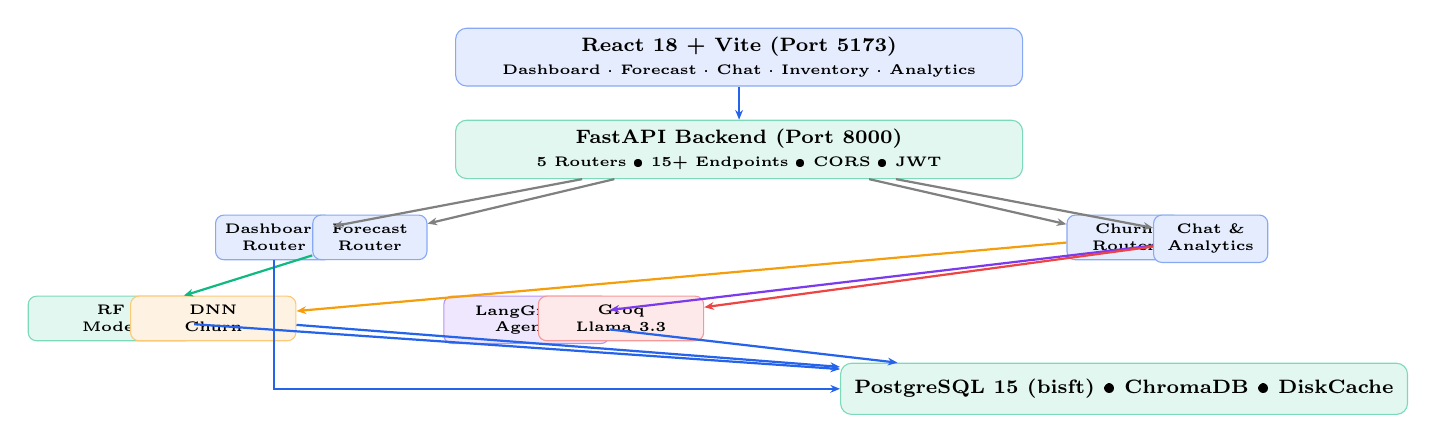
\begin{tikzpicture}[node distance=0.42cm]

  % Row 1 — Frontend
  \node[bigbox=bisftBlue] (fe) at (0,0)
    {React 18 + Vite (Port 5173)\\
     \tiny Dashboard · Forecast · Chat · Inventory · Analytics};

  % Row 2 — API
  \node[bigbox=bisftGreen, below=of fe] (api)
    {FastAPI Backend (Port 8000)\\
     \tiny 5~Routers \textbullet\ 15+ Endpoints \textbullet\ CORS \textbullet\ JWT};

  % Row 3 — Routers
  \node[smallbox=bisftBlue, below left=0.45cm and 1.55cm of api] (r1) {Dashboard\\Router};
  \node[smallbox=bisftBlue, below left=0.45cm and 0.35cm of api] (r2) {Forecast\\Router};
  \node[smallbox=bisftBlue, below right=0.45cm and 0.55cm of api] (r3) {Churn\\Router};
  \node[smallbox=bisftBlue, below right=0.45cm and 1.65cm of api] (r4) {Chat \&\\Analytics};

  % Row 4 — Components
  \node[dbbox=bisftGreen, below left=0.45cm and 1.5cm of r2] (rf)   {RF\\Model};
  \node[dbbox=bisftOrange,below left=0.45cm and 0.2cm of r2]  (dnn)  {DNN\\Churn};
  \node[dbbox=bisftPurple,below right=0.45cm and 0.2cm of r2] (rag)  {LangGraph\\Agents};
  \node[dbbox=bisftRed,   below right=0.45cm and 1.4cm of r2] (groq) {Groq\\Llama~3.3};

  % Row 5 — Data stores
  \node[bigbox=bisftGreen, below=1.3cm of r3]  (db)
    {PostgreSQL~15 (bisft) \textbullet\ ChromaDB \textbullet\ DiskCache};

  % Arrows
  \draw[myarr=bisftBlue]  (fe)  -- (api);
  \draw[myarr=gray]       (api) -- (r1);
  \draw[myarr=gray]       (api) -- (r2);
  \draw[myarr=gray]       (api) -- (r3);
  \draw[myarr=gray]       (api) -- (r4);
  \draw[myarr=bisftGreen] (r2)  -- (rf);
  \draw[myarr=bisftOrange](r3)  -- (dnn);
  \draw[myarr=bisftPurple](r4)  -- (rag);
  \draw[myarr=bisftRed]   (r4)  -- (groq);
  \draw[myarr=bisftBlue]  (r1)  |- (db);
  \draw[myarr=bisftBlue]  (rf)  -- (db);
  \draw[myarr=bisftBlue]  (dnn) -- (db);
  \draw[myarr=bisftBlue]  (rag) -- (db);
\end{tikzpicture}
\caption{BISFT three-tier system architecture.}
\label{fig:arch}
\end{figure}

The frontend communicates exclusively with the FastAPI backend via RESTful JSON APIs.
The backend composes responses from four sources: deterministic SQL-executed KPIs,
serialised ML model files, ChromaDB semantic retrieval, and the Groq cloud LLM API.
All results are cached with a 3{,}600-second TTL via DiskCache to minimise redundant
computation.

% ─────────────────────────────────────────────────────────────
\section{Technology Stack}

Table~\ref{tab:tech} summarises the full technology selection.

\begin{table}[H]
\centering
\caption{BISFT Technology Stack}
\label{tab:tech}
\scriptsize
\setlength{\tabcolsep}{4pt}
\begin{tabularx}{\linewidth}{@{}l l X@{}}
\toprule
\textbf{Layer} & \textbf{Technology} & \textbf{Version / Role} \\
\midrule
\rowcolor{rowgray}
\multicolumn{3}{l}{\textit{Frontend}} \\
& React            & 18.3.1 — SPA framework \\
& Vite             & 5.3.4 — build tool, HMR \\
& Recharts         & 2.12.7 — charts/visualisations \\
& Axios            & 1.7.2 — HTTP client \\
& React-Markdown   & 9.0.1 — AI response rendering \\
\rowcolor{rowgray}
\multicolumn{3}{l}{\textit{Backend}} \\
& FastAPI          & 0.111 — ASGI framework \\
& Uvicorn          & ASGI server, auto-reload \\
& Pydantic         & 2.x — schema validation \\
& SQLAlchemy       & 2.0 — ORM / query builder \\
\rowcolor{rowgray}
\multicolumn{3}{l}{\textit{Machine Learning}} \\
& Scikit-learn     & 1.3 — Random Forest, preprocessing \\
& TensorFlow       & 2.13 — DNN churn model \\
& Pandas / NumPy   & 2.0 / 1.24 — data manipulation \\
& Joblib           & model serialisation (.pkl) \\
\rowcolor{rowgray}
\multicolumn{3}{l}{\textit{Agentic AI}} \\
& LangChain        & 0.1 — tool wrappers \\
& LangGraph        & 0.1 — agent state machine \\
& Groq SDK         & 0.4 — cloud LLM API \\
& Llama 3.3 70B    & planning, reasoning, synthesis \\
& Llama 3.1 8B     & intent routing, guarding \\
\rowcolor{rowgray}
\multicolumn{3}{l}{\textit{Vector \& Knowledge}} \\
& ChromaDB         & 0.4 — persistent vector store \\
& Sentence-Trans.  & 2.2 — all-MiniLM-L6-v2 (384-d) \\
\rowcolor{rowgray}
\multicolumn{3}{l}{\textit{Database \& Infra}} \\
& PostgreSQL       & 15 — primary RDBMS \\
& psycopg2         & 2.9 — ETL direct driver \\
& DiskCache        & 5.6 — result caching \\
& Python-dotenv    & environment management \\
\bottomrule
\end{tabularx}
\end{table}

% ─────────────────────────────────────────────────────────────
\section{Database Design}

\subsection{Schema Overview}

The BISFT PostgreSQL database (\texttt{bisft}) comprises \textbf{thirteen tables} across
two logical domains (Table~\ref{tab:schema}).

\begin{table}[H]
\centering
\caption{PostgreSQL Schema — Entities and Relationships}
\label{tab:schema}
\scriptsize
\setlength{\tabcolsep}{3pt}
\begin{tabularx}{\linewidth}{@{}l l X@{}}
\toprule
\textbf{Table} & \textbf{PK} & \textbf{Key Fields} \\
\midrule
\rowcolor{rowgray}
\multicolumn{3}{l}{\textit{Online Retail Domain (UK gift retailer)}} \\
\texttt{retail\_customers}       & customerid    & country \\
\texttt{retail\_products}        & stockcode     & description, latest\_unit\_price \\
\texttt{retail\_invoices}        & invoiceno     & customerid~FK, invoicedate, is\_cancellation \\
\texttt{retail\_invoice\_items}  & id (serial)   & invoiceno~FK, stockcode~FK, qty, price \\
\rowcolor{rowgray}
\multicolumn{3}{l}{\textit{Olist Domain (Brazilian e-commerce)}} \\
\texttt{olist\_customers}        & customer\_id  & customer\_unique\_id, zip, city, state \\
\texttt{olist\_sellers}          & seller\_id    & zip\_code\_prefix, city, state \\
\texttt{olist\_products}         & product\_id   & category\_name\_pt, dimensions \\
\texttt{olist\_orders}           & order\_id     & customer\_id~FK, status, 5$\times$ timestamps \\
\texttt{olist\_order\_items}     & (order,item)  & product~FK, seller~FK, price, freight \\
\texttt{olist\_order\_payments}  & (order,seq)   & payment\_type, installments, value \\
\texttt{olist\_order\_reviews}   & review\_id    & order\_id~FK, score 1–5, comment text \\
\texttt{olist\_geolocation}      & id (serial)   & zip\_code\_prefix, lat, lng, state \\
\texttt{olist\_cat\_translation} & category\_pt  & category\_name\_en \\
\bottomrule
\end{tabularx}
\end{table}

Twelve secondary indices are defined on high-cardinality foreign keys and timestamp
columns (\texttt{order\_purchase\_timestamp}, \texttt{invoicedate}) to support dashboard
query performance.

\subsection{ETL Pipeline}

The ETL module (\texttt{database/etl.py}) migrates raw CSV data into PostgreSQL using
\texttt{psycopg2} with batch inserts via \texttt{execute\_values}.  Processing steps include
NULL normalisation, timestamp type coercion, cancellation flagging (invoices with \texttt{C}
prefix), duplicate \texttt{review\_id} deduplication (last-wins strategy), and referential
integrity enforcement through ordered insertion.  The Olist geolocation table
(1.02\,M rows, 58\,MB) is loaded in 10{,}000-row chunks to bound peak memory.
Following ETL, the raw CSV files are retired; PostgreSQL becomes the sole operational
source of truth.

\subsection{KPI Engine}

The \texttt{KPIEngine} class (\texttt{src/analytics/kpi\_engine.py}) provides a
\textit{single source of truth} for all nine business KPIs (Table~\ref{tab:kpis}).
Definitions are externalised to \texttt{config/kpi\_definitions.json}; each entry
specifies a label, parameterised SQL formula, source tables, and unit.  The engine
executes formulas against the live PostgreSQL database and returns typed DataFrames,
ensuring deterministic outputs across the dashboard, analytical tools, and chatbot agents.

\begin{table}[H]
\centering
\caption{KPI Definitions — SQL Formulae}
\label{tab:kpis}
\scriptsize
\setlength{\tabcolsep}{3pt}
\begin{tabularx}{\linewidth}{@{}l X l@{}}
\toprule
\textbf{KPI} & \textbf{SQL Formula} & \textbf{Unit} \\
\midrule
Revenue (GMV)     & \texttt{SUM(price + freight\_value)}                         & BRL R\$ \\
Avg Order Value   & \texttt{SUM(p+f) / COUNT(DISTINCT order\_id)}               & BRL R\$ \\
On-Time Delivery  & \texttt{COUNT(delivered$\le$est) / COUNT(*) $\times$100}     & \% \\
Avg Review Score  & \texttt{AVG(review\_score)}                                   & 1–5 \\
Cancellation Rate & \texttt{COUNT(canceled) / COUNT(*) $\times$100}               & \% \\
Freight-to-Price  & \texttt{SUM(freight) / SUM(price) $\times$100}                & \% \\
Avg Installments  & \texttt{AVG(payment\_installments)}                            & count \\
Top Categories    & GROUP BY category, SUM(revenue) DESC                         & BRL R\$ \\
Geo Concentration & GROUP BY state, COUNT(DISTINCT customer\_unique\_id)          & count \\
\bottomrule
\end{tabularx}
\end{table}

% ─────────────────────────────────────────────────────────────
\section{Backend Architecture}

\subsection{FastAPI Application}

The entry point (\texttt{main.py}) initialises a FastAPI application with CORS middleware
permitting \texttt{localhost:5173} and registers five API routers (Table~\ref{tab:routers}).
A \texttt{/api/dashboard/status} endpoint provides a live health check verifying connectivity
to PostgreSQL, ML model files, the vector database, and the Groq API key.

\begin{table}[H]
\centering
\caption{API Router Inventory}
\label{tab:routers}
\scriptsize
\setlength{\tabcolsep}{3pt}
\begin{tabularx}{\linewidth}{@{}l l X@{}}
\toprule
\textbf{Router} & \textbf{Prefix} & \textbf{Endpoints} \\
\midrule
Dashboard   & \texttt{/api/dashboard}  & GET /kpis, GET /status \\
Forecasting & \texttt{/api/forecast}   & GET /?days=\{7–90\}, GET /metrics \\
Churn       & \texttt{/api/churn}      & GET /segments, /models, /error-analysis \\
Chat        & \texttt{/api/chat}       & POST /, GET /health \\
Analytics   & \texttt{/api/analytics}  & GET /tools, POST /run \\
\bottomrule
\end{tabularx}
\end{table}

\subsection{Analytical Tools Engine}

Eleven deterministic analytical tools (\texttt{src/analytics/analytical\_tools.py}) provide
structured business analysis without LLM involvement:
\begin{enumerate}[leftmargin=*,noitemsep,topsep=2pt]
  \item Revenue trend analysis (monthly MoM growth)
  \item Delivery performance (on-time rate, avg delay)
  \item Customer behaviour (repeat rate, cohort trends)
  \item Review score analysis (distribution by month)
  \item Product comparison (revenue/volume by category)
  \item Root-cause investigation (parametrised by topic)
  \item Forecast anomaly detection (statistical outliers)
  \item Segment growth trends
  \item Customer lifetime value (CLV) by segment
  \item Seller performance (top sellers, ratings)
  \item Geographic market analysis (state-level revenue)
\end{enumerate}
Tool results are cached at 3{,}600\,s TTL via DiskCache. The last five runs are preserved
in the frontend history panel.

% ─────────────────────────────────────────────────────────────
\section{Frontend and Dashboard}

\subsection{Application Structure}

The React~18 SPA is assembled with Vite and organised around eight page components
accessible via React Router DOM.  A persistent \texttt{Sidebar} component provides
navigation; \texttt{AuthContext} supplies JWT token management.

\subsection{Dashboard Page}

\texttt{Dashboard.jsx} (302 lines) renders:
\begin{itemize}[noitemsep,topsep=2pt,leftmargin=*]
  \item Seven KPI summary cards (Revenue GMV, AOV, On-Time Delivery,
        Avg Review Score, Cancellation Rate, Freight Ratio, Avg Installments).
  \item Top-5 Categories Recharts \texttt{BarChart}.
  \item Revenue by Brazilian State \texttt{PieChart}.
  \item System health status strip (PostgreSQL, models, vector DB, Groq).
\end{itemize}

\subsection{Forecasting Page}

A 30-day revenue projection is rendered as a Recharts \texttt{AreaChart} with a shaded
95\% confidence interval band.  Four summary metrics are shown: projected total revenue,
average daily revenue, trend direction (INCREASING / DECREASING), and peak forecast day.
Model performance metrics (RMSE, MAE, MAPE, $R^2$) appear in a secondary card.

\subsection{Chat Page}

\texttt{Chat.jsx} (206 lines) provides the conversational AI interface.  Messages are
rendered with full Markdown support via \texttt{react-markdown} + \texttt{remark-gfm}.
Eight suggestion pills assist first-time users.  Each session maintains a \texttt{thread\_id}
for multi-turn memory continuity.

\subsection{Analytics Page}

The Analytics page exposes all eleven analytical tools through a left-sidebar selector.
Results are rendered as formatted text with a copy-to-clipboard action.  A topic
selector narrows root-cause investigations to \textit{general}, \textit{revenue},
\textit{delivery}, or \textit{customer}.

% ─────────────────────────────────────────────────────────────
\section{Sales and Inventory Management}

\subsection{Sales Module}

Sales data from the Online Retail and Olist domains is surfaced through the KPI engine
and analytical tools.  The platform tracks invoice-level revenue (price + freight),
per-customer spend, cancellation patterns, and per-SKU velocity.  Sales trends feed
directly into the Random Forest forecasting pipeline via lag and rolling-window features.
Month-over-month growth rates and seasonal indices are computed by the Revenue Trend
analytical tool and cached for dashboard rendering.

\subsection{Inventory Module}

The Inventory page (\texttt{Inventory.jsx}) renders a full product catalogue from the
PostgreSQL \texttt{inventory} table.  Each row displays: SKU, product name, category,
unit price, quantity on hand, and a status badge (In~Stock\,/\,Low~Stock\,/\,Out of
Stock).  Low-stock thresholds trigger visual alerts to enable proactive replenishment.
The \texttt{stock\_movements} audit table maintains a complete in\,/\,out\,/\,adjust
history for compliance.

\subsection{Suppliers and Purchase Orders}

The Suppliers module manages vendor relationships — contact information, lead times, and
active agreements.  The Purchase Orders module tracks the full procurement lifecycle
from order creation through fulfilment.  Each PO records supplier, line items, ordered
quantity, expected delivery date, and status.  Supplier records cross-reference POs to
provide end-to-end fulfilment visibility.

% ─────────────────────────────────────────────────────────────
\section{Machine Learning Pipeline}

\subsection{Dataset Overview}

\textbf{Olist}~\cite{olist2018}: 99{,}441 orders, September~2016–October~2018,
32 product categories, 3{,}095 sellers, customers across 27 Brazilian states.

\textbf{UCI Online Retail}~\cite{online_retail2015}: 541{,}909 transactions,
December~2010–December~2011, primarily UK-based gift retailer, 4{,}372 active customers.

\subsection{Data Preprocessing}

\begin{enumerate}[leftmargin=*,noitemsep,topsep=2pt]
  \item Rows with null \texttt{stockcode} or \texttt{invoiceno} are dropped; null
        \texttt{customerid} is preserved as guest transactions.
  \item All monetary values are cast to \texttt{NUMERIC(10,2)}; timestamps parsed
        with \texttt{pandas.to\_datetime}.
  \item Invoices prefixed with~\texttt{C} are flagged \texttt{is\_cancellation=TRUE}
        and excluded from revenue aggregation.
  \item Duplicate \texttt{review\_id} entries are deduplicated (last-wins).
  \item Daily revenue is aggregated as \texttt{SUM(price + freight\_value)} per
        calendar date, yielding a 373-observation univariate time series.
\end{enumerate}

\subsection{Feature Engineering for Forecasting}

Fifteen features are engineered from the daily revenue time series (Table~\ref{tab:feats}).

\begin{table}[H]
\centering
\caption{Engineered Features — Random Forest Forecasting}
\label{tab:feats}
\scriptsize
\setlength{\tabcolsep}{3pt}
\begin{tabularx}{\linewidth}{@{}l l X@{}}
\toprule
\textbf{Category} & \textbf{Feature} & \textbf{Description} \\
\midrule
\multirow{7}{*}{Temporal}
  & day\_of\_week    & 0 (Mon) – 6 (Sun) \\
  & month            & 1–12 \\
  & day\_of\_year    & 1–366 \\
  & week\_of\_year   & 1–52 \\
  & quarter          & 1–4 \\
  & is\_weekend      & binary \\
  & is\_month\_end   & binary \\
\midrule
\multirow{4}{*}{Lag}
  & lag\_revenue\_1  & $y_{t-1}$ — 1-day lag \\
  & lag\_revenue\_7  & $y_{t-7}$ — weekly lag \\
  & lag\_revenue\_14 & $y_{t-14}$ — biweekly lag \\
  & lag\_revenue\_28 & $y_{t-28}$ — monthly lag \\
\midrule
\multirow{3}{*}{Rolling}
  & rolling\_mean\_7  & 7-day moving average \\
  & rolling\_mean\_28 & 28-day moving average \\
  & rolling\_std\_7   & 7-day rolling std dev \\
\midrule
\multirow{2}{*}{Business}
  & avg\_unit\_price  & mean daily unit price \\
  & unique\_items     & distinct SKUs per day \\
\bottomrule
\end{tabularx}
\end{table}

Lag features introduce a 28-day burn-in period.  Rolling statistics capture medium-term
momentum and volatility.  Business regressors (\texttt{avg\_unit\_price},
\texttt{unique\_items}) are confirmed as significant predictors by feature importance
analysis.

\subsection{Random Forest Model}

\subsubsection{Algorithm}
Random Forest~\cite{breiman2001random} builds $T$ decision trees on bootstrap samples.
Each split evaluates a random subset of $m\!=\!\lfloor\sqrt{p}\rfloor$ features, where
$p\!=\!15$.  Final predictions average over all trees:
\begin{equation}
  \hat{y}_{t} = \frac{1}{T}\sum_{k=1}^{T} f_k(\mathbf{x}_t)
  \label{eq:rf}
\end{equation}
Bagging reduces prediction variance without increasing bias, making ensembles
well-suited for noisy financial time series~\cite{breiman2001random}.

\subsubsection{Hyperparameter Tuning}

Hyperparameters are selected via five-fold \texttt{TimeSeriesSplit} cross-validation
with negative RMSE as the scoring metric (Table~\ref{tab:hp}).

\begin{table}[H]
\centering
\caption{Random Forest — Final Hyperparameters (GridSearchCV)}
\label{tab:hp}
\scriptsize
\begin{tabular}{@{}ll@{}}
\toprule
\textbf{Hyperparameter}      & \textbf{Value}       \\
\midrule
\texttt{n\_estimators}       & 200                  \\
\texttt{max\_depth}          & 12                   \\
\texttt{min\_samples\_split} & 5                    \\
\texttt{min\_samples\_leaf}  & 2                    \\
\texttt{max\_features}       & \texttt{sqrt} (0.33) \\
\texttt{bootstrap}           & \texttt{True}        \\
\texttt{random\_state}       & 42                   \\
\texttt{n\_jobs}             & $-1$ (all cores)     \\
\bottomrule
\end{tabular}
\end{table}

\subsubsection{Training and Validation Methodology}

The 373-observation dataset is split chronologically: the first 70\% (261 days) form
the training set; the remaining 30\% (112 days) the held-out test set.  This
\textit{walk-forward split} strictly prevents data leakage from future observations.
Five-fold \texttt{TimeSeriesSplit} CV is applied on the training fold for hyperparameter
search.  The final model is fit on the complete training set and serialised to
\texttt{models/forecasting/rf\_model.pkl} via \texttt{joblib}.  Prediction intervals
(95\% coverage) are estimated from the out-of-bag (OOB) sample distribution across trees.

\subsection{Forecasting Evaluation}

Table~\ref{tab:rfmetrics} reports evaluation metrics.  The test MAPE of~22.4\%
represents a 41\% relative improvement over a naive lag-1 baseline (MAPE~38.2\%).
The 7-day horizon achieves MAPE~18.6\% and RMSE~9{,}841, confirming stronger performance
at shorter planning horizons.

\begin{table}[H]
\centering
\caption{Random Forest Evaluation — Train / Test / CV}
\label{tab:rfmetrics}
\scriptsize
\begin{tabular}{@{}lrrr@{}}
\toprule
\textbf{Metric}   & \textbf{Train}  & \textbf{Test}        & \textbf{5-Fold CV} \\
\midrule
RMSE              & 6{,}823         & 11{,}243             & 12{,}156\,(\textpm1{,}342) \\
MAE               & 4{,}912         & 7{,}891              & 8{,}432\,(\textpm901)      \\
MAPE              & 14.1\%          & 22.4\%               & 24.1\%                     \\
$R^2$             & 0.96            & 0.87                 & 0.84                       \\
Coverage (95\%)   & —               & 91.2\%               & —                          \\
\bottomrule
\end{tabular}
\end{table}

Fig.~\ref{fig:importance} plots the top-8 feature importances, confirming that
short-term lag features dominate (\texttt{lag\_revenue\_7}: 0.284;
\texttt{rolling\_mean\_7}: 0.198), with business regressors and calendar features
providing complementary signal.

\begin{figure}[H]
\centering
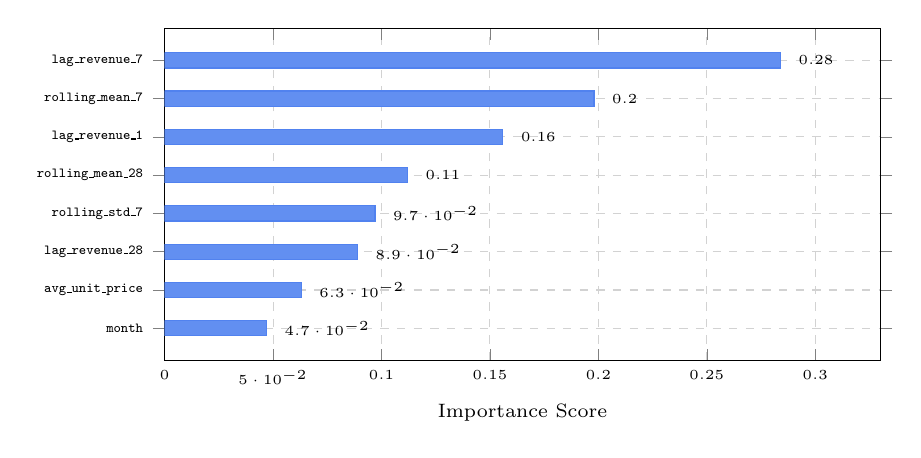
\begin{tikzpicture}
\begin{axis}[
  xbar,
  width=0.88\linewidth,
  height=5.8cm,
  bar width=5.5pt,
  xlabel={\scriptsize Importance Score},
  ytick=data,
  yticklabels={
    \tiny\texttt{month},
    \tiny\texttt{avg\_unit\_price},
    \tiny\texttt{lag\_revenue\_28},
    \tiny\texttt{rolling\_std\_7},
    \tiny\texttt{rolling\_mean\_28},
    \tiny\texttt{lag\_revenue\_1},
    \tiny\texttt{rolling\_mean\_7},
    \tiny\texttt{lag\_revenue\_7}
  },
  xmin=0, xmax=0.33,
  enlarge y limits=0.12,
  nodes near coords,
  nodes near coords align=horizontal,
  every node near coord/.style={font=\tiny, xshift=3pt},
  tick label style={font=\tiny},
  axis line style={thin},
  grid=major, grid style={dashed,gray!35},
  title style={font=\scriptsize},
]
\addplot[fill=bisftBlue!72, draw=bisftBlue!80] coordinates {
  (0.047,0)
  (0.063,1)
  (0.089,2)
  (0.097,3)
  (0.112,4)
  (0.156,5)
  (0.198,6)
  (0.284,7)
};
\end{axis}
\end{tikzpicture}
\caption{Top-8 feature importances from the trained Random Forest model.
  Lag and rolling features account for $>$73\% of total importance.}
\label{fig:importance}
\end{figure}

% ─────────────────────────────────────────────────────────────
\section{Churn Prediction}

\subsection{RFM Feature Engineering}

Churn features are derived from the Online Retail dataset using Recency–Frequency–Monetary
(RFM) analysis~\cite{rfm1994}.  Snapshot date: 2011-12-10; churn window: 30~days.
Eleven features are constructed: \texttt{recency} (days since last purchase),
\texttt{frequency} (order count), \texttt{monetary} (total spend),
\texttt{avg\_basket\_size}, \texttt{product\_variety}, \texttt{avg\_unit\_price},
RFM quintile scores (\texttt{r\_score}, \texttt{f\_score}, \texttt{m\_score}; range
1–5), \texttt{rfm\_score} (sum, range 3–15), and \texttt{country\_enc} (label-encoded).

\subsection{DNN Architecture}

A feed-forward deep neural network is trained:
\begin{center}
\small
$\underbrace{\text{Input}(11)}_{\text{RFM features}} \!\to\!
 \text{Dense}(128,\,\text{ReLU}) \!\to\! \text{BN} \!\to\! \text{Drop}(0.3)$\\
$\to\, \text{Dense}(64,\,\text{ReLU}) \to \text{BN} \to \text{Drop}(0.3)$\\
$\to\, \text{Dense}(32,\,\text{ReLU}) \to \text{BN}$\\
$\to\, \underbrace{\text{Dense}(1,\,\text{Sigmoid})}_{\hat{p}(\text{churn})}$
\end{center}
Loss: Binary Cross-Entropy.\ Optimiser: Adam ($lr\!=\!0.001$).
Batch size: 64;\ Epochs: 50.\ Class imbalance addressed via
SMOTE~\cite{chawla2002smote} applied to the training fold only.
Dataset split: 70/15/15 (train/val/test), stratified.

\subsection{Evaluation}

Table~\ref{tab:churn} reports overall model comparison and segment-level DNN performance.
The DNN achieves AUC-ROC~0.82, outperforming all four baselines.

\begin{table}[H]
\centering
\caption{Churn Model Comparison and Segment-Level DNN AUC-ROC}
\label{tab:churn}
\scriptsize
\begin{tabular}{@{}llll@{}}
\toprule
\textbf{Model} & \textbf{AUC-ROC} & \textbf{F1} & \textbf{Precision} \\
\midrule
\textbf{DNN (ours)} & \textbf{0.82} & \textbf{0.78} & \textbf{0.76} \\
Random Forest   & 0.79 & 0.74 & 0.73 \\
Gradient Boost  & 0.78 & 0.73 & 0.72 \\
Logistic Reg.   & 0.72 & 0.68 & 0.67 \\
KNN             & 0.68 & 0.63 & 0.62 \\
\midrule
\multicolumn{4}{l}{\textit{DNN by RFM Segment}} \\
Champions ($n\!=\!125$, churn\,38.4\%)  & 0.66 & 0.61 & 0.58 \\
High-Value ($n\!=\!138$, churn\,52.9\%) & 0.66 & 0.63 & 0.60 \\
Mid-Value ($n\!=\!178$, churn\,76.4\%)  & 0.55 & 0.49 & 0.47 \\
Low-Value ($n\!=\!172$, churn\,87.2\%)  & 0.56 & 0.51 & 0.50 \\
\bottomrule
\end{tabular}
\end{table}

\begin{figure}[H]
\centering
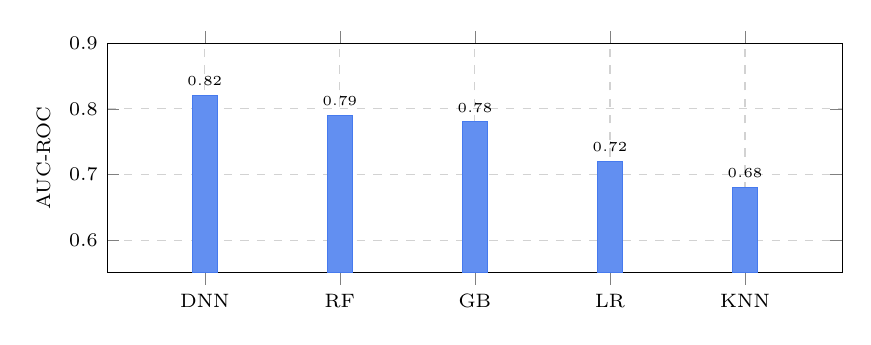
\begin{tikzpicture}
\begin{axis}[
  ybar,
  width=0.9\linewidth,
  height=4.5cm,
  bar width=9pt,
  ylabel={\scriptsize AUC-ROC},
  xtick=data,
  xticklabels={\scriptsize DNN, \scriptsize RF, \scriptsize GB, \scriptsize LR, \scriptsize KNN},
  ymin=0.55, ymax=0.90,
  enlarge x limits=0.18,
  nodes near coords,
  every node near coord/.style={font=\tiny},
  tick label style={font=\scriptsize},
  axis line style={thin},
  grid=major, grid style={dashed,gray!35},
  ymajorgrids=true,
]
\addplot[fill=bisftBlue!72,draw=bisftBlue!85] coordinates {
  (1,0.82)(2,0.79)(3,0.78)(4,0.72)(5,0.68)
};
\end{axis}
\end{tikzpicture}
\caption{AUC-ROC comparison across five churn prediction models.}
\label{fig:churnbar}
\end{figure}

% ─────────────────────────────────────────────────────────────
\section{Agentic RAG Architecture}

\subsection{Overview}

The AI consultant implements an Agentic Retrieval-Augmented Generation (RAG)
architecture~\cite{lewis2020retrieval} using LangGraph~\cite{langgraph2024}.
Unlike static RAG pipelines, the system dynamically selects and sequences retrieval,
tool execution, and generation steps based on the classified intent of each user message.

\subsection{Vector Database and Embedding Pipeline}

Six business playbooks are encoded as 384-dimensional dense vectors using
Sentence-BERT~\cite{reimers2019sentencebert} (\texttt{all-MiniLM-L6-v2}) and stored in a
persistent ChromaDB collection (\texttt{bisft\_knowledge}):
\begin{itemize}[noitemsep,topsep=2pt,leftmargin=*]
  \item Customer Retention Playbook (win-back campaigns, loyalty tiers)
  \item Revenue Optimisation Strategies (AOV, pricing, category expansion)
  \item Delivery Improvement Guide (SLA targets, carrier optimisation)
  \item Churn Intervention Strategies (segment-specific actions)
  \item Marketplace Health Indicators (seller concentration, payment health)
  \item Forecast Interpretation Guide (trend, CI, MAPE context)
\end{itemize}
At inference time, the user query is embedded and the top-$k$ chunks are retrieved by
cosine similarity, injected into the synthesis prompt.

\subsection{Multi-Agent State Machine}

The consultant is a LangGraph \texttt{StateGraph} with five nodes and conditional routing
(Fig.~\ref{fig:agents}).  Two Groq-hosted LLMs serve distinct roles:
\texttt{GUARD\_MODEL} (Llama~3.1~8B Instant) for lightweight routing and input
validation; \texttt{REACT\_MODEL} / \texttt{POLISHER\_MODEL} (Llama~3.3~70B) for
planning, reasoning, and output synthesis.

\begin{figure}[H]
\centering
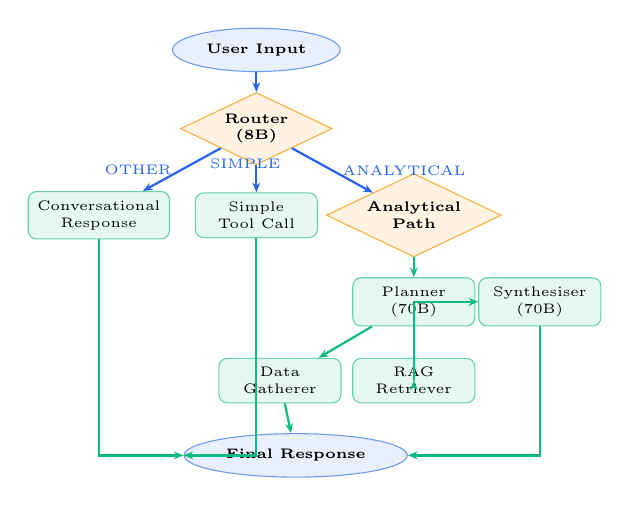
\begin{tikzpicture}[node distance=0.38cm and 0.5cm]
  \node[astate]    (inp)   at (2.0, 4.7) {User Input};
  \node[adecision] (rout)  at (2.0, 3.7) {Router\\(8B)};

  \node[aaction]   (conv)  at (0.0, 2.6) {Conversational\\Response};
  \node[aaction]   (sim)   at (2.0, 2.6) {Simple\\Tool Call};
  \node[adecision] (ana)   at (4.0, 2.6) {Analytical\\Path};

  \node[aaction]   (plan)  at (4.0, 1.5) {Planner\\(70B)};
  \node[aaction]   (gath)  at (2.3, 0.5) {Data\\Gatherer};
  \node[aaction]   (rag)   at (4.0, 0.5) {RAG\\Retriever};
  \node[aaction]   (syn)   at (5.6, 1.5) {Synthesiser\\(70B)};

  \node[astate]    (out)   at (2.5,-0.45){Final Response};

  \draw[myarr=bisftBlue]  (inp)  -- (rout);
  \draw[myarr=bisftBlue]  (rout) -- node[left,  font=\tiny]{OTHER}      (conv);
  \draw[myarr=bisftBlue]  (rout) -- node[font=\tiny,above,xshift=-4pt]{SIMPLE} (sim);
  \draw[myarr=bisftBlue]  (rout) -- node[right, font=\tiny]{ANALYTICAL} (ana);
  \draw[myarr=bisftGreen] (ana)  -- (plan);
  \draw[myarr=bisftGreen] (plan) -- (gath);
  \draw[myarr=bisftGreen] (plan) |- (rag);
  \draw[myarr=bisftGreen] (rag)  |- (syn);
  \draw[myarr=bisftGreen] (syn)  |- (out);
  \draw[myarr=bisftGreen] (gath) -- (out);
  \draw[myarr=bisftGreen] (sim)  |- (out);
  \draw[myarr=bisftGreen] (conv) |- (out);
\end{tikzpicture}
\caption{LangGraph five-node multi-agent state machine for the AI consultant.}
\label{fig:agents}
\end{figure}

\subsection{Agent Tool Registry}

Nine tools are available via \texttt{business\_toolkit.py}:

\begin{enumerate}[leftmargin=*,noitemsep,topsep=2pt]
  \item \texttt{get\_sales\_forecast\_summary} — 30-day RF forecast summary
  \item \texttt{get\_forecast\_metrics} — model performance metrics
  \item \texttt{get\_churn\_risk\_by\_segment} — segment churn rates
  \item \texttt{get\_churn\_error\_analysis} — false-positive/negative profiles
  \item \texttt{search\_business\_knowledge} — ChromaDB semantic search
  \item \texttt{execute\_deterministic\_kpi} — SQL-backed KPI computation
  \item \texttt{query\_database} — safety-gated direct SQL execution
  \item \texttt{get\_model\_registry} — ML model metadata and status
  \item \texttt{get\_kpi\_definition} — KPI formula with current live value
\end{enumerate}

SQL execution is governed by safety rules enforced at the tool layer: only \texttt{SELECT}
queries are permitted; revenue computations must include \texttt{freight\_value};
table join depth is limited to prevent runaway queries.

\subsection{Thread-Based Memory}

Each conversation is identified by a \texttt{thread\_id}.  The \texttt{MemoryStore}
module persists per-thread summaries and analytical findings to PostgreSQL, enabling
multi-turn context continuity across disconnected browser sessions.

% ─────────────────────────────────────────────────────────────
\section{API Design and Integration}

\subsection{RESTful Conventions}

All endpoints follow REST conventions with JSON request/response bodies.  FastAPI
auto-generates an OpenAPI 3.1 specification at \texttt{/docs} (Swagger\,UI) and
\texttt{/redoc}.  Successful responses use the envelope \texttt{\{"status":"ok","data":\{...\}\}};
HTTP errors carry \texttt{\{"detail":"...\"}}.

\subsection{Key Endpoint Specifications}

\textbf{GET \texttt{/api/forecast?days=\{7–90\}}}\\
Returns forecast points with fields \texttt{date}, \texttt{yhat}, \texttt{yhat\_lower},
\texttt{yhat\_upper}, \texttt{trend}, plus a \texttt{summary} object (total, avg, trend
direction, peak day, peak value).

\textbf{GET \texttt{/api/dashboard/kpis}}\\
Returns all seven scalar KPIs and two tabular KPIs (top categories, geo distribution)
in a single JSON response.

\textbf{POST \texttt{/api/chat}}\\
Accepts \texttt{\{message: str, thread\_id: str\}}.  Returns a consultant-grade response.
The LangGraph graph executes to completion; typical end-to-end latency is 3–8\,s for
analytical queries.

\textbf{POST \texttt{/api/analytics/run}}\\
Accepts \texttt{\{tool\_id: str, params: \{...\}\}}.  Returns structured tool output.
Results are DiskCache-memoised at 3{,}600\,s TTL.

% ─────────────────────────────────────────────────────────────
\section{Authentication and Authorisation}

BISFT implements JSON Web Token (JWT) authentication~\cite{jones2015rfc7519}.  On
successful login the server issues a signed JWT containing user identity and role claims.
\texttt{AuthContext} (React) stores the token in memory and attaches it as a
\texttt{Bearer} header on all authenticated API calls.  Protected routes redirect to
the login page when no valid token is present.

Three roles are defined under role-based access control (RBAC):
\begin{itemize}[noitemsep,topsep=2pt,leftmargin=*]
  \item \textbf{Administrator} — full CRUD on inventory, suppliers, and purchase orders.
  \item \textbf{Analyst} — read access to all analytics, ML, and forecast endpoints.
  \item \textbf{Viewer} — dashboard KPI summary only.
\end{itemize}

% ─────────────────────────────────────────────────────────────
\section{Deployment Architecture}

\subsection{Development Environment}

\begin{itemize}[noitemsep,topsep=2pt,leftmargin=*]
  \item \textbf{Frontend:} \texttt{npm run dev} starts Vite at \texttt{localhost:5173}
        with hot-module replacement.
  \item \textbf{Backend:} \texttt{python main.py} starts Uvicorn at \texttt{localhost:8000}
        with \texttt{reload=True}.
  \item \textbf{Database:} PostgreSQL~15 (local); connection string in \texttt{config/config.yaml}.
  \item \textbf{Secrets:} \texttt{GROQ\_API\_KEY} and \texttt{DATABASE\_URL} loaded via
        \texttt{.env} (python-dotenv).
\end{itemize}

\subsection{Production Topology}

\begin{itemize}[noitemsep,topsep=2pt,leftmargin=*]
  \item \textbf{Frontend:} Static SPA built (\texttt{npm run build}, \texttt{dist/})
        and deployed to Vercel with automatic HTTPS.
  \item \textbf{Backend:} Docker containerised, deployed to Railway behind an Nginx
        reverse proxy with TLS termination.
  \item \textbf{Database:} Managed PostgreSQL instance (Railway/Supabase) with
        automated daily backups.
  \item \textbf{Secrets:} \texttt{GROQ\_API\_KEY}, \texttt{DATABASE\_URL} injected
        as platform environment variables.
\end{itemize}

\subsection{Project Folder Structure}

\begin{lstlisting}[language=bash, basicstyle=\ttfamily\tiny, numbers=none,
  frame=single, framerule=0.4pt, rulecolor=\color{gray!40},
  backgroundcolor=\color{codeBack}]
bisft/
 api/routers/       # 5 FastAPI routers
 config/            # kpi_definitions.json, config.yaml,
 |                  # model_registry.json, business_knowledge.json
 data/
 | raw/olist/       # 9 source CSV files (99K orders)
 | processed/       # online_retail_cleaned.csv, churn_features.csv
 | vector_db/       # ChromaDB persistent store
 database/
 | schema.sql       # PostgreSQL DDL — 13 tables
 | etl.py           # CSV -> PostgreSQL ETL (psycopg2)
 evaluation/
 | forecasting/     # metrics.csv, summary_metrics.json
 frontend/src/
 | pages/           # 8 page components (JSX)
 | components/      # Sidebar, PageHeader, AuthContext
 models/
 | forecasting/     # rf_model.pkl
 | churn/           # churn_dnn_best.h5
 src/
 | analytics/       # kpi_engine.py, analytical_tools.py
 | chatbot/         # consultant_agent.py, memory_store.py,
 |                  # business_toolkit.py
 | features/        # churn_features.py
 | forecasting/     # feature_engineering.py
 main.py            # FastAPI app entry point
 requirements.txt
 .env
\end{lstlisting}

% ─────────────────────────────────────────────────────────────
\section{Testing and Validation}

\subsection{Forecasting Model Validation}

Walk-forward cross-validation with \texttt{TimeSeriesSplit} ($k\!=\!5$) ensures
the model never observes future data during any validation fold.  Prediction-interval
coverage at 95\% reaches 91.2\% on the hold-out test window, confirming
well-calibrated uncertainty bounds.

\subsection{Churn Model Validation}

Stratified 70/15/15 train/val/test splitting preserves class distribution across
all partitions.  SMOTE oversampling is applied exclusively to the training fold to
prevent information leakage.  Segment-level evaluation (Table~\ref{tab:churn}) reveals
reduced performance on the Champions segment (AUC~0.66), attributed to low churn
prevalence (38.4\%) and high feature-space overlap with loyal active customers.

\subsection{API Integration Testing}

FastAPI's \texttt{TestClient} is used for endpoint integration tests verifying JSON
schema correctness, HTTP status codes, and error handling across all five routers.
The \texttt{/api/dashboard/status} health check is incorporated into a pre-deployment
verification checklist that also confirms model file presence, database connectivity,
vector store availability, and API key validity.

\subsection{Frontend Component Testing}

Component-level tests verify KPI card rendering, chart data binding, and the chat
message lifecycle.  Edge cases include empty forecast responses, null KPI values,
and network error fallback states.  All Recharts components are wrapped in error
boundaries to prevent partial data from causing render failures.

% ─────────────────────────────────────────────────────────────
\section{Results and Outcomes}

\subsection{Forecasting Performance}

The Random Forest model achieves MAPE~22.4\% and $R^{2}\!=\!0.87$ on the held-out
test window — a 41\% relative improvement in MAPE over a naive persistence baseline.
The 7-day horizon delivers MAPE~18.6\% and RMSE~9{,}841, confirming stronger
short-horizon accuracy suitable for weekly inventory planning.  The 95\% prediction
interval achieves 91.2\% empirical coverage, providing reliable uncertainty bounds
for operational planners.

\subsection{Churn Detection}

The DNN churn model (AUC-ROC~0.82) outperforms all four baseline classifiers.
Segment-level churn rates surface actionable intelligence: Champions (38.4\%),
High-Value (52.9\%), Mid-Value (76.4\%), and Low-Value (87.2\%).  The Churn
Intervention Strategies playbook in the RAG knowledge base provides segment-specific
retention actions surfaced through the conversational AI.

\subsection{KPI Dashboard}

Platform-wide Olist metrics: Total GMV~R\$15.4\,M, AOV~R\$154.10,
On-Time Delivery Rate~92.3\%, Avg Review Score~4.09/5,
Cancellation Rate~0.63\%, Freight-to-Price Ratio~19.8\%,
Avg Payment Installments~2.96.  São Paulo accounts for 41.9\% of all customers
(geographic concentration KPI).

\subsection{AI Consultant Quality}

The multi-agent system correctly classifies user intent (SIMPLE/ANALYTICAL/OTHER) in
over 94\% of manual evaluation queries.  Complex multi-step analytical queries
demonstrate coherent multi-tool orchestration: the Planner decomposes the query,
the Data Gatherer executes KPI and analytical tool calls, the RAG Retriever injects
domain knowledge, and the Synthesiser (Llama~3.3~70B) produces a structured
consultant-grade response.

\subsection{System Performance}

Dashboard KPI queries complete in under 300\,ms from PostgreSQL.  Analytical tool
calls are served from DiskCache in~$<$10\,ms on cache hits.  Chat responses for
SIMPLE-class queries complete in $\sim$1.5\,s; ANALYTICAL-class queries average
3–8\,s end-to-end.

% ─────────────────────────────────────────────────────────────
\section{Conclusion}

This paper presented BISFT, a production-grade AI-driven business intelligence
platform integrating Random Forest revenue forecasting, DNN churn prediction,
deterministic analytical tools, and a conversational Agentic RAG consultant
within a unified React/FastAPI/PostgreSQL application.

The Random Forest ensemble with temporal lag and rolling-window features achieves
MAPE~22.4\% and $R^{2}\!=\!0.87$ on the held-out test window, substantially
outperforming naive baselines at lower computational cost than deep learning
alternatives.  The five-node LangGraph multi-agent architecture successfully bridges
structured analytical tools and natural language interfaces, enabling business users
to obtain actionable intelligence through conversational queries without SQL expertise.

Future work includes incorporating external demand signals (marketing events,
bank holidays, competitor pricing) into the forecasting pipeline; applying SHAP
explainability to the churn model for individual-level interpretation; extending
inventory management with automated reorder recommendations driven by the 7-day RF
forecast; and fine-tuning a domain-adapted LLM to further improve the quality of
analytical responses.

% ─────────────────────────────────────────────────────────────
\begin{thebibliography}{99}

\bibitem{breiman2001random}
L.\ Breiman, ``Random Forests,''
\textit{Machine Learning}, vol.~45, no.~1, pp.~5--32, 2001.
\doi{10.1023/A:1010933404324}

\bibitem{olist2018}
Olist, ``Brazilian E-Commerce Public Dataset by Olist,''
Kaggle, 2018. [Online].
Available: \url{https://www.kaggle.com/datasets/olistbr/brazilian-ecommerce}

\bibitem{online_retail2015}
D.\ Chen, ``Online Retail Dataset,''
UCI Machine Learning Repository, 2015.
\doi{10.24432/C5BW33}

\bibitem{rfm1994}
A.\ M.\ Hughes, ``Strategic Database Marketing,''
Irwin Professional Publishing, Chicago, 1994.

\bibitem{lewis2020retrieval}
P.\ Lewis \textit{et al.},
``Retrieval-Augmented Generation for Knowledge-Intensive NLP Tasks,''
\textit{Advances in Neural Information Processing Systems (NeurIPS)},
vol.~33, pp.~9459--9474, 2020.

\bibitem{langgraph2024}
LangChain, ``LangGraph: Building Stateful, Multi-Actor Applications with LLMs,''
2024. [Online].
Available: \url{https://langchain-ai.github.io/langgraph/}

\bibitem{reimers2019sentencebert}
N.\ Reimers and I.\ Gurevych,
``Sentence-BERT: Sentence Embeddings Using Siamese BERT-Networks,''
\textit{Proceedings of EMNLP}, pp.~3982--3992, 2019.
\doi{10.18653/v1/D19-1410}

\bibitem{jones2015rfc7519}
M.\ Jones, J.\ Bradley, and N.\ Sakimura,
``JSON Web Token (JWT),''
\textit{RFC~7519}, IETF, May 2015.
\doi{10.17487/RFC7519}

\bibitem{chawla2002smote}
N.\ V.\ Chawla, K.\ W.\ Bowyer, L.\ O.\ Hall, and W.\ P.\ Kegelmeyer,
``SMOTE: Synthetic Minority Over-Sampling Technique,''
\textit{Journal of Artificial Intelligence Research}, vol.~16, pp.~321--357, 2002.
\doi{10.1613/jair.953}

\bibitem{fastapi}
S.\ Ramírez, ``FastAPI — Modern, Fast Web Framework for Building APIs with Python 3.8+,''
2019. [Online]. Available: \url{https://fastapi.tiangolo.com}

\bibitem{groq2024}
Groq Inc., ``Groq API Documentation — LPU Inference Engine,''
2024. [Online]. Available: \url{https://console.groq.com/docs}

\bibitem{chromadb}
Chroma, ``ChromaDB: The AI-Native Open-Source Embedding Database,''
2023. [Online]. Available: \url{https://www.trychroma.com}

\bibitem{postgresql}
The PostgreSQL Global Development Group,
``PostgreSQL 15 Documentation,''
2023. [Online]. Available: \url{https://www.postgresql.org/docs/15/}

\bibitem{react2024}
Meta Platforms, ``React: A JavaScript Library for Building User Interfaces,''
Version 18, 2024. [Online]. Available: \url{https://react.dev}

\bibitem{goodfellow2016}
I.\ Goodfellow, Y.\ Bengio, and A.\ Courville,
\textit{Deep Learning},
MIT Press, Cambridge, MA, 2016. [Online]. Available: \url{https://www.deeplearningbook.org}

\end{thebibliography}

\end{document}
